\documentclass[10pt]{beamer}
\setbeamerfont{normal text}{size=\small}
\AtBeginDocument{\usebeamerfont{normal text}}

\usefonttheme{professionalfonts}

\usetheme[progressbar=frametitle]{metropolis}
\usepackage{appendixnumberbeamer}

\usepackage{booktabs}
\usepackage[scale=2]{ccicons}

\usepackage{pgfplots}
\usepgfplotslibrary{dateplot}

\usepackage{xspace}
\newcommand{\themename}{\textbf{\textsc{metropolis}}\xspace}

\title{Gatsby Bridging Program}
\subtitle{Probability: Discrete Distributions}
% \date{\today}
\date{}
\author{Cameron Stewart}
\institute{Gatsby Computational Neuroscience Unit}
\titlegraphic{\hfill
\includegraphics[height=1.5cm]{logo.png}}

\begin{document}

\maketitle

\begin{frame}{Today's Lecture Topics}
  \setbeamertemplate{section in toc}[sections numbered]
  \tableofcontents%[hideallsubsections]
\end{frame}

\section{Random Variables, Probability Mass Functions, and Cumulative Distribution Functions}

\begin{frame}[fragile]{What is a Random Variable?}
Random variables are functions which map the possible outcomes of an experiment to numerical values. In general, for random variable \(X\) and sample space \(\Omega\), we have that \(X: \Omega \rightarrow \mathbb{R}\).
\onslide<2>{\metroset{block=fill}\begin{exampleblock}{Example 1}
Consider a bag containing 3 red balls (R) and 5 green balls (G). In our experiment, we are going to draw 2 balls from the bag, with replacement. The sample space is \(\Omega = \left\{\textrm{RR}, \textrm{RG}, \textrm{GR}, \textrm{GG}\right\}\).

We are interested in determining the probabilities of drawing various numbers of red balls. To do this, we could start by defining a random variable \(X: \Omega \rightarrow \left\{0, 1, 2\right\}\) such that
\begin{equation*}
    X\left(\omega\right) =
    \begin{cases}
        0 & \textrm{if } \omega = \textrm{GG}\\
        1 & \textrm{if } \omega \in \left\{\textrm{RG, GR}\right\}\\
        2 & \textrm{if } \omega = \textrm{RR}
    \end{cases}\,.
\end{equation*}
\end{exampleblock}}
\end{frame}

\begin{frame}[fragile]{What is a Random Variable?}
Random variables are often utilised without any explicit reference to the sample space. Instead of writing \(X\left(\omega\right)\), we will typically just write \(X\). Instead of writing \(\mathbb{P}\left(E\right)\) for some event \(E\), we typically write \(\mathbb{P}\left(X \in A\right)\) for some set of numerical values \(A\). To be precise, \(\mathbb{P}\left(X \in A\right) = \mathbb{P}\left(\left\{\omega \in \Omega \;\middle|\; X\left(\omega\right) \in A\right\}\right)\).
\onslide<2>{\metroset{block=fill}\begin{exampleblock}{Example 1 Cont.}
What is the probability of drawing one red ball? We could express this as \(\mathbb{P}\left(\left\{\textrm{RG, GR}\right\}\right)\), but it is common and accepted notation to instead write \(\mathbb{P}\left(X \in \left\{1\right\}\right)\), or \(\mathbb{P}\left(0 < X < 2\right)\), or most preferably in this case \(\mathbb{P}\left(X = 1\right)\).
\begin{equation*}\begin{aligned}
    \mathbb{P}\left(X = 1\right) &= \mathbb{P}\left(\left\{\textrm{RG}\right\} \cup \left\{\textrm{GR}\right\}\right)\\
    &= \mathbb{P}\left(\left\{\textrm{RG}\right\}\right) + \mathbb{P}\left(\left\{\textrm{GR}\right\}\right) - \mathbb{P}\left(\left\{\textrm{RG}\right\} \cap \left\{\textrm{GR}\right\}\right)\\
    &= \mathbb{P}\left(\left\{\textrm{RR}, \textrm{RG}\right\}\right)\mathbb{P}\left(\left\{\textrm{RG}, \textrm{GG}\right\}\right) + \mathbb{P}\left(\left\{\textrm{GR}, \textrm{GG}\right\}\right)\mathbb{P}\left(\left\{\textrm{RR}, \textrm{GR}\right\}\right)\\
    &= \frac{3}{8}\frac{5}{8} + \frac{5}{8}\frac{3}{8}\,.
\end{aligned}\end{equation*}
\end{exampleblock}}
\end{frame}

\begin{frame}[fragile]{The Chain Rule and Independence}
In a previous lecture, we covered the following relationship for events \(E\) and \(F\):
\begin{equation*}\begin{aligned}
    \mathbb{P}\left(E \cap F\right) &= \mathbb{P}\left(E \;\middle|\; F\right)\mathbb{P}\left(F\right)\\
    &= \mathbb{P}\left(F \;\middle|\; E\right)\mathbb{P}\left(E\right)\,.
\end{aligned}\end{equation*}
\onslide<2->{This also applies to random variables. Here we are looking at the probability of random variables \(X\) and \(Y\) taking values in sets \(A\) and \(B\) respectively, which of course corresponds to the probability of two events:
\metroset{block=fill}\begin{alertblock}{Chain Rule for Two Random Variables}
\begin{equation*}
\begin{aligned}
    \overbrace{\mathbb{P}\left(X \in A, Y \in B\right)}^{\substack{\textrm{Joint}\\\textrm{Probability}}} &= \overbrace{\mathbb{P}\left(X \in A \;\middle|\; Y \in B\right)}^{\substack{\textrm{Conditional}\\\textrm{Probability}}}\overbrace{\mathbb{P}\left(Y \in B\right)}^{\substack{\textrm{Marginal}\\\textrm{Probability}}}\\
    &= \mathbb{P}\left(Y \in B \;\middle|\; X \in A\right)\mathbb{P}\left(X \in A\right)
\end{aligned}
\end{equation*}
\end{alertblock}}
\onslide<3>{A future lecture will cover joint, conditional, and marginal distributions and the chain rule, independence, and marginalisation in more detail.}
\end{frame}

\begin{frame}[fragile]{The Chain Rule and Independence}
In this lecture, we will only consider independent random variables. For two random variables to be independent, the realisation of one must have no effect on the distribution of the other. E.g. a coin flip is independent of the outcome of the previous coin flip.\onslide<2->{ Mathematically, we write this as
\begin{equation*}
    \mathbb{P}\left(X \in A, Y \in B\right) = \mathbb{P}\left(X \in A\right)\mathbb{P}\left(Y \in B\right)\,,
\end{equation*}
taking note that independence implies
\begin{equation*}
    \mathbb{P}\left(X \in A \;\middle|\; Y \in B\right) = \mathbb{P}\left(X \in A\right)\,.
\end{equation*}}
\onslide<3>{For \(n\) independent random variables, this generalises to:
\metroset{block=fill}\begin{alertblock}{Independence of \(n\) Random Variables}
\begin{equation*}
    \mathbb{P}\left(X_1 \in A_1, \dots, X_n \in A_n\right) = \prod_{i=1}^n\mathbb{P}\left(X_i \in A_i\right)
\end{equation*}\end{alertblock}}
\end{frame}

\begin{frame}[fragile]{The Chain Rule and Independence}
\metroset{block=fill}\begin{exampleblock}{Example 1 Cont.}
In our red ball example, we could also use separate random variables for the outcomes of each draw from the bag. Let \(X_1 \in \left\{0, 1\right\}\) be the random variable representing the first draw and \(X_2 \in \left\{0, 1\right\}\) be the random variable representing the second draw (0 for a green ball and 1 for red ball). Then it is straightforward to see that \(X = X_1 + X_2\).

\onslide<2->{Are \(X_1\) and \(X_2\) independent?}\onslide<3->{ Yes, they are independent random variables, as the first draw has no effect on the second draw.}

\onslide<4->{What if we had the same experimental setup, but without replacing the ball after the first draw?}\onslide<5>{ In this case they are not independent, as the colour of the first drawn ball will dictate the probabilities of the second drawn ball.}
\end{exampleblock}
\end{frame}

\begin{frame}[fragile]{The Chain Rule and Independence}
\textit{A hint for the problem set questions:}

Whilst we won't be dealing with dependent random variables today, some problem set questions will still require you to work with conditional probabilities. Take note that
\begin{equation*}
    \mathbb{P}\left(X \in A \;\middle|\; X \in B\right) = \frac{\mathbb{P}\left(X \in A, X \in B\right)}{\mathbb{P}\left(X \in B\right)}\,.
\end{equation*}
There is nothing special about this. We are simply looking at the probability of one event conditioned on the occurrence of another.
\end{frame}

\begin{frame}[fragile]{Discrete and Continuous Random Variables}
Discrete random variables can take a countable number of values. For example:
\begin{itemize}
    \item \(X \in \left\{0, 1\right\}\)
    \item \(X \in \left\{0, 1, 2, \dots\right\}\)
    \item \(X\) representing the number of buses arriving within an hour.
\end{itemize}

\onslide<2>{Continuous random variables can take values in continuous ranges. For example:
\begin{itemize}
    \item \(X \in \left[0, 1\right]\)
    \item \(X \in \mathbb{R}\)
    \item \(X\) representing the waiting time until the next bus.
\end{itemize}}
\end{frame}

\begin{frame}[fragile]{Probability Mass Functions}
Discrete distributions can be defined by their probability mass function (PMF). The PMF of random variable \(X\) is often denoted by \(f_X\) or \(p_X\), and is defined as:
\metroset{block=fill}\begin{alertblock}{Probability Mass Functions}
\begin{equation*}
    f_X\left(x\right) = \mathbb{P}\left(X = x\right)
\end{equation*}
\end{alertblock}
\onslide<2>{\(f_X\) is simply a function name. It is fine to use a different name, as long as it is clear how the function is defined. Occasionally, the same name is used for PMFs if it is clear from context how these are defined, but I'd advise against this practice for the sake of clarity. E.g. it is clearer to write \(p_X\left(x\right)\) and \(p_Y\left(y\right)\) than \(p\left(x\right)\) and \(p\left(y\right)\) if these correspond to 2 different PMFs.}
\end{frame}

\begin{frame}[fragile]{Probability Mass Functions}
Probabilities can't be negative and must sum to 1 over the set of all possible values \(\mathcal{X}\), so we have the following constraints:
\begin{equation*}
    f_X\left(x\right) \geq 0 \textrm{ for all } x
\end{equation*}
and
\begin{equation*}
    \sum_{x \in \mathcal{X}} f_X\left(x\right) = 1\,.
\end{equation*}
\(\mathcal{X}\) is referred to as the support of \(X\). \(f_X\left(x\right) = 0\) for \(x \notin \mathcal{X}\).
\end{frame}

\begin{frame}[fragile]{Probability Mass Functions}
\metroset{block=fill}\begin{exampleblock}{Example 1 Cont.}
Let's continue with our red ball example. What is the PMF of \(X\)? First, we recognise that \(\mathcal{X} = \left\{0, 1, 2\right\}\). You can verify for yourself that
\begin{equation*}
    f_X\left(x\right) =
    \begin{cases}
        \frac{25}{64} & \textrm{if } x = 0\\
        \frac{15}{32} & \textrm{if } x = 1\\
        \frac{9}{64} & \textrm{if } x = 2\\
        0 & \textrm{otherwise}
    \end{cases}\,,
\end{equation*}
and that this function satisfies the conditions for a PMF on the previous slide.
\end{exampleblock}
\end{frame}

\begin{frame}[fragile]{Probability Mass Functions}
Often, we use a \(\sim\) to mean "is distributed as". It is very common to see the notation
\begin{equation*}
    X \sim f_x\,,
\end{equation*}
which, in the discrete case, means that \(X\) has the PMF \(f_x\). Variations of this notation exist, but there should never be any ambiguity about the distribution of a random variable when using a \(\sim\).

\onslide<2>{Sometimes you will see
\begin{equation*}
    X_1, \dots, X_n \overset{\textrm{i.i.d.}}{\sim} f_x\,,
\end{equation*}
which implies that all \(n\) random variables are independent and identically distributed (i.i.d.) with PMF \(f_x\).}
\end{frame}

\begin{frame}[fragile]{Cumulative Distribution Functions}
A probability distribution can also be defined in terms of its cumulative distribution function (CDF). The CDF of a random variable \(X\) is a monotonically increasing function defined as:
\metroset{block=fill}\begin{alertblock}{Cumulative Distribution Functions}
\begin{equation*}
    F_X\left(x\right) = \mathbb{P}\left(X \leq x\right)
\end{equation*}
\end{alertblock}
\onslide<2>{For discrete random variables, we can relate this definition to the PMF as follows:
\begin{equation*}
    F_X\left(x\right) = \sum_{y\leq x} f_X\left(y\right)\,.
\end{equation*}}
\end{frame}

\begin{frame}[fragile]{Cumulative Distribution Functions}
As probabilities must sum to 1 over the support, we have the following emergent properties for CDFs:
\begin{equation*}\begin{aligned}
    \lim_{x\rightarrow-\infty}F_X\left(x\right) = 0\\
    \lim_{x\rightarrow\infty}F_X\left(x\right) = 1
\end{aligned}\end{equation*}
\onslide<2>{We can also see that the following is true:
\begin{equation*}
\begin{aligned}
    \mathbb{P}\left(a < X \leq b\right) &= \mathbb{P}\left(X \leq b\right) - \mathbb{P}\left(X \leq a\right)\\
    &= F_X\left(b\right) - F_X\left(a\right)\,.
\end{aligned}
\end{equation*}}
\end{frame}

\begin{frame}[fragile]{Cumulative Distribution Functions}
\metroset{block=fill}\begin{exampleblock}{Example 1 Cont.}
Back to the red ball example. What is the CDF of \(X\)? Previously, we found that
\begin{equation*}
    f_X\left(x\right) =
    \begin{cases}
        \frac{25}{64} & \textrm{if } x = 0\\
        \frac{15}{32} & \textrm{if } x = 1\\
        \frac{9}{64} & \textrm{if } x = 2\\
        0 & \textrm{otherwise}
    \end{cases}\,.
\end{equation*}
Hence, the CDF is
\begin{equation*}
    F_X\left(x\right) =
    \begin{cases}
        0 & \textrm{if } x < 0\\
        \frac{25}{64} & \textrm{if } 0 \leq x < 1\\
        \frac{55}{64} & \textrm{if } 1 \leq x < 2\\
        1 & \textrm{if } x \geq 2
    \end{cases}\,.
\end{equation*}
\end{exampleblock}
\end{frame}

\begin{frame}[fragile]{PDF and CDF Plots}
\metroset{block=fill}\begin{exampleblock}{Example 1 Cont.}
\begin{columns}
\begin{column}{0.425\textwidth}
\begin{figure}
    \centering
    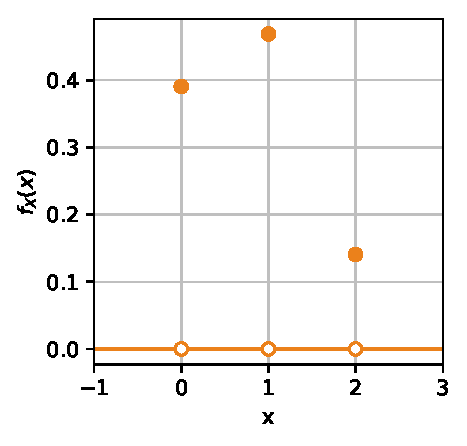
\includegraphics[width=\textwidth]{pmf.eps}
    \caption{Probability Mass Function}
\end{figure}
\end{column}
\begin{column}{0.425\textwidth}
\begin{figure}
    \centering
    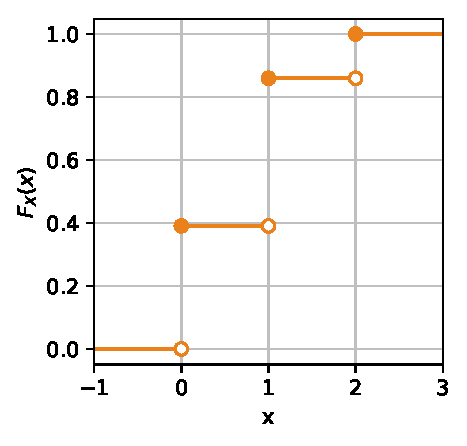
\includegraphics[width=\textwidth]{cdf.eps}
    \caption{Cumulative Distribution Function}
\end{figure}
\end{column}
\end{columns}
\end{exampleblock}
\end{frame}

\begin{frame}[fragile]{Sampling}
Similarly to how we refer to realisations of random variables, we can also talk about samples of distributions. Sampling from a discrete distribution with PMF \(f_x\) simply implies that we randomly generate a number \(x\) with probability \(f_x\left(x\right)\).

\onslide<2->{To be entirely correct, drawing \(n\) samples from \(f_x\) involves running \(n\) random experiments with \(n\) associated random variables \(X_1, \dots, X_n \overset{\textrm{i.i.d.}}{\sim} f_x\) and generating \(n\) realisations \(x_1, \dots, x_n\).}

\onslide<3>{As \(n \rightarrow \infty\), we will observe that
\begin{equation*}
    \frac{\sum_{i = 1}^n \href{https://en.wikipedia.org/wiki/Iverson_bracket}{\color{mLightBrown}{\left[x_i = x\right]}}}{n} \rightarrow f_x\left(x\right)
\end{equation*}}
\end{frame}

\begin{frame}[standout]
Intermission
\end{frame}

\section{Expectation and Variance}

\begin{frame}[fragile]{Expectations}
Suppose we want to know the average value of a function \(g\left(x\right)\) evaluated at samples from a distribution. More precisely, we wish to draw realisations of \(X_1, \dots, X_n \overset{\textrm{i.i.d.}}{\sim} f_x\) and then compute the mean of \(\left\{g\left(x_1\right), \dots, g\left(x_n\right)\right\}\). As \(n\) increases, this will converge to a value which we call the expectation (or expected value). This theorem is referred to as the law of large numbers.

\onslide<2->{We can estimate the expectation for finite \(n\) as follows:
\metroset{block=fill}\begin{alertblock}{Empirical Estimates of Expectations}
\begin{equation*}
    \underset{X \sim f_X}{\mathbb{E}}\left[g\left(X\right)\right] \approx \frac{1}{n}\sum_{i = 1}^n g\left(x_i\right)\qquad\textrm{for large }n
\end{equation*}
\end{alertblock}}
\end{frame}

\begin{frame}[fragile]{Expectations}
If \(X\) is discrete with support \(\mathcal{X}\) and PMF \(f_X\), we can also define this expectation as a weighted average:
\metroset{block=fill}\begin{alertblock}{Expectations on Discrete Distributions}
\begin{equation*}
    \underset{X \sim f_X}{\mathbb{E}}\left[g\left(X\right)\right] = \sum_{x \in \mathcal{X}} f_X\left(x\right)g\left(x\right)
\end{equation*}
\end{alertblock}

\onslide<2->{If the distribution on which the expectation is taken is clear from context, the text under the \(\mathbb{E}\) is often omitted.}

\onslide<3>{When talking about the mean of a distribution defined by \(f_X\), this specifically refers to the value given by
\begin{equation*}
    \underset{X \sim f_X}{\mathbb{E}}\left[X\right]\,.
\end{equation*}}
\end{frame}

\begin{frame}[fragile]{Properties of Expectations}
\begin{itemize}[<+->]
    \item Linearity:
        \begin{equation*}
            \mathbb{E}\left[ag\left(X\right) + bh\left(X\right)\right] = a\mathbb{E}\left[g\left(X\right)\right] + b\mathbb{E}\left[h\left(X\right)\right]\,,
        \end{equation*}
        for constants \(a, b\) and functions \(g, h\).
    \item Non-multiplicativity:
        In general,
        \begin{equation*}
            \mathbb{E}\left[g\left(X\right)h\left(X\right)\right] \neq \mathbb{E}\left[g\left(X\right)\right]\mathbb{E}\left[h\left(X\right)\right]\,.
        \end{equation*}
    \item \(\mathbb{E}\left[a\right] = a\) for constant \(a\). Hence, \(\mathbb{E}\left[\mathbb{E}\left[X\right]\right] = \mathbb{E}\left[X\right]\).
\end{itemize}
\onslide<4>{\href{https://en.wikipedia.org/wiki/Expected_value\#Properties}{\color{mLightBrown}{Additional properties}} exist for multivariate distributions.}
\end{frame}

\begin{frame}[fragile]{Expectations}
\metroset{block=fill}\begin{exampleblock}{Example 2}
Suppose we roll a six-sided die. Let \(X \in \left\{1, 2, 3, 4, 5, 6\right\}\) represent this roll. What is the expected value of \(X\)?

\onslide<2->{Firstly, we define the support as \(\mathcal{X} \in \left\{1, 2, 3, 4, 5, 6\right\}\) and the PMF \(f_X\) as
\begin{equation*}
f_X\left(x\right) =
\begin{cases}
    \frac{1}{6} & \textrm{if } x \in \mathcal{X}\\
    0 & \textrm{otherwise}
\end{cases}\,.
\end{equation*}}

\onslide<3>{Then the expected value of \(X\) is given by
\begin{equation*}
\begin{aligned}
    \mathbb{E}\left[X\right] &= \sum_{x \in \mathcal{X}} f_X\left(x\right)x\\
    &= \frac{1}{6}\cdot 1 + \frac{1}{6}\cdot 2 + \frac{1}{6}\cdot 3 + \frac{1}{6}\cdot 4 + \frac{1}{6}\cdot 5 + \frac{1}{6}\cdot 6\\
    &= 3.5
\end{aligned}
\end{equation*}}
\end{exampleblock}
\end{frame}

\begin{frame}[fragile]{Expectations}
Why care about expectations?
\begin{itemize}[<+->]
    \item A huge number of statistical estimation problems, where we try to estimate model parameters given some data, can be written in terms of expectations.
    \item This includes machine learning problems. Training a machine learning model involves minimising a loss function. The loss function and its gradient is very often written in terms of expectations.
    \item We can approximate these expectations simply by drawing samples!
\end{itemize}
\end{frame}

\begin{frame}[fragile]{Variance}
How about if we want to know how "spread out" a distribution is? A way of measuring this is with the variance. It measures the expected deviation from the mean.
\metroset{block=fill}\begin{alertblock}{Variance of a Random Variable}
\begin{equation*}\begin{aligned}
    \textrm{Var}\left(X\right) &= \mathbb{E}\left[\left(X - \mathbb{E}\left[X\right]\right)^2\right]\\
    &= \mathbb{E}\left[X^2 - 2X\mathbb{E}\left[X\right] + \mathbb{E}\left[X\right]^2\right]\\
    &= \mathbb{E}\left[X^2\right] - 2\mathbb{E}\left[X\right]\mathbb{E}\left[X\right] + \mathbb{E}\left[X\right]^2\\
    &= \mathbb{E}\left[X^2\right] - \mathbb{E}\left[X\right]^2
\end{aligned}\end{equation*}
\end{alertblock}
\end{frame}

\begin{frame}[fragile]{Properties of Variance}
\begin{itemize}[<+->]
    \item \(\textrm{Var}\left(aX + b\right) = a^2\textrm{Var}\left(X\right)\) for constants \(a, b\).
    \item \(\textrm{Var}\left(a\right) = 0\) for constant \(a\).
    \item \(\textrm{Var}\left(X\right) \geq 0\).
\end{itemize}
\onslide<4>{\href{https://en.wikipedia.org/wiki/Variance\#Properties}{\color{mLightBrown}{Additional properties}} exist for multivariate distributions.}
\end{frame}

\begin{frame}[fragile]{Variance}
\metroset{block=fill}\begin{exampleblock}{Example 2 Cont.}
    Continuing with the die roll example. What is the variance of \(X\)?

\onslide<2->{We will compute the variance of \(X\) in two separate ways. Method 1:
\begin{equation*}
\begin{aligned}
    \textrm{Var}\left(X\right) &= \mathbb{E}\left[\left(X - \mathbb{E}\left[X\right]\right)^2\right]\\
     &= \mathbb{E}\left[\left(X - 3.5\right)^2\right]\\
     &= \sum_{x \in \mathcal{X}} f_X\left(x\right)\left(x - 3.5\right)^2\\
     &= \frac{1}{6}\left(1 - 3.5\right)^2 + \frac{1}{6}\left(2 - 3.5\right)^2 + \frac{1}{6}\left(3 - 3.5\right)^2 + \frac{1}{6}\left(4 - 3.5\right)^2\\
     &\phantom{=}\quad + \frac{1}{6}\left(5 - 3.5\right)^2 + \frac{1}{6}\left(6 - 3.5\right)^2\\
     &= 2.91\dot{6}
\end{aligned}
\end{equation*}}
\end{exampleblock}
\end{frame}

\begin{frame}[fragile]{Variance}
\metroset{block=fill}\begin{exampleblock}{Example 2 Cont.}
Method 2:
\begin{equation*}\begin{aligned}
    \textrm{Var}\left(X\right) &= \mathbb{E}\left[X^2\right] - \mathbb{E}\left[X\right]^2\\
     &= \sum_{x \in \mathcal{X}} f_X\left(x\right)x^2 - 3.5^2\\
     &= \frac{1}{6}\cdot 1^2 + \frac{1}{6}\cdot 2^2 + \frac{1}{6}\cdot 3^2 + \frac{1}{6}\cdot 4^2 + \frac{1}{6}\cdot 5^2 + \frac{1}{6}\cdot 6^2 - 3.5^2\\
     &= 2.91\dot{6}
\end{aligned}\end{equation*}
\end{exampleblock}
\end{frame}

\begin{frame}[fragile]{Notation}
It is typical to see the notations \(\mu\), \(\sigma^2\), and \(\sigma\) used for the mean, variance, and standard deviation of a distribution respectively. Clearly, the standard deviation is just the square root of the variance. In other words, we have:
\begin{equation*}\begin{aligned}
    \mu &= \mathbb{E}\left[X\right]\\
    \sigma^2 &= \textrm{Var}\left(X\right)\,.
\end{aligned}\end{equation*}
\end{frame}

\begin{frame}[standout]
Intermission
\end{frame}

\section{Important Discrete Distributions}

\begin{frame}[fragile]{Why Study Specific Distributions?}
\begin{itemize}[<+->]
    \item Many real-world scenarios can be modelled with a few simple distributions. E.g. modelling the chance of success, the number of successes in a finite number of trials, the number of failures until a success, the waiting time until an event happens, and the uncertainty in an estimate after multiple measurements.
    \item A large number of these simple distributions have very nice mathematical properties, including important relationships between them.
\end{itemize}

\onslide<3>{After the lecture on continuous distributions, I'd recommend doing some \href{http://www.math.wm.edu/~leemis/chart/UDR/UDR.html}{\color{mLightBrown}{exploring}} of these distributions and their relationships.}
\end{frame}

\begin{frame}[fragile]{Functions of Random Variables}
The next few slides will deal with simple functions of random variables. We have an entire lecture later on which will cover this topic in much more depth. For now, all you need to know are the following:
\begin{itemize}[<+->]
    \item Functions of random variables are also random variables. E.g. if \(g\) is a function and \(X, Y\) are random variables, then \(Z = g\left(X, Y\right)\) is also a random variable. The distribution of \(Z\) can often be pretty complicated!
    \item The realisation of \(Z\) is given by the realisations of \(X\) and \(Y\) passed through \(g\). I.e. \(z = g\left(x, y\right)\). So sampling can often be pretty easy!
\end{itemize}\onslide<3>{

\textit{A hint for the problem set questions:}

If \(X\) and \(Y\) are discrete and independent, then \(Z = X + Y\) has the PMF
\begin{equation*}
    f_Z\left(z\right) = \sum_{x \in \mathcal{X}}f_X\left(x\right)f_Y\left(z - x\right)\,.
\end{equation*}
You may use this without proof. A summation of this form is called a convolution.}
\end{frame}

\begin{frame}[fragile]{Discrete Uniform Distribution}
If a random variable takes any integer between \(a\) and \(b\) inclusive with equal probability, then it follows a discrete uniform distribution.

\metroset{block=fill}\begin{alertblock}{Discrete Uniform Distribution}
Discrete uniform random variable \(X \sim \mathcal{U}\left\{a, b\right\}\) has the following properties:
  \begin{table}
    \begin{tabular}{ll}
      \toprule
      Parameters & \(a, b \in \mathbb{Z} \mid b \geq a\)\\
      Support & \(\mathcal{X} = \{a,\dots, b\}\)\\
      PMF & \(f_X\left(x\right) = \frac{1}{b - a + 1}\qquad\textrm{for }x \in \mathcal{X}\)\\
      Mean & \(\mathbb{E}\left[X\right] = \frac{a + b}{2}\)\\
      Variance & \(\textrm{Var}\left(X\right) = \frac{\left(b - a + 1\right)^2 - 1}{12}\)\\
      \bottomrule
    \end{tabular}
  \end{table}
\end{alertblock}
\end{frame}

\begin{frame}[fragile]{Discrete Uniform Distribution}
\metroset{block=fill}\begin{exampleblock}{Example 2 Cont.}
Back to the die roll example. Is \(X\) uniformly distributed?

\onslide<2->{Yes, it is uniformly distributed with \(a = 1\) and \(b = 6\).}\onslide<3>{ We can easily confirm our previous calculations with the formulas on the last slide:
\begin{equation*}
\begin{aligned}
    \mathbb{E}\left[X\right] &= \frac{1 + 6}{2}\\
    &= 3.5
\end{aligned}
\end{equation*}
and
\begin{equation*}
\begin{aligned}
    \textrm{Var}\left(X\right) &= \frac{(6 - 1 + 1)^2 - 1}{12}\\
    &= 2.91\dot{6}\,.
\end{aligned}
\end{equation*}}
\end{exampleblock}
\end{frame}

\begin{frame}[fragile]{Bernoulli Distribution}
If a random variable takes the value \(1\) with probability \(p\), and \(0\) otherwise, then it follows a Bernoulli distribution. It models the probability of "success".

\metroset{block=fill}\begin{alertblock}{Bernoulli Distribution}
Bernoulli random variable \(X \sim \textrm{Bern}\left(p\right)\) has the following properties:
  \begin{table}
    \begin{tabular}{ll}
      \toprule
      Parameters & \(p \in \left[0,1\right]\)\\
      Support & \(\mathcal{X} = \{0,1\}\)\\
      PMF & \(f_X\left(x\right) = p^x\left(1 - p\right)^{1 - x}\qquad\textrm{for }x \in \mathcal{X}\)\\
      Mean & \(\mathbb{E}\left[X\right] = p\)\\
      Variance & \(\textrm{Var}\left(X\right) = p\left(1 - p\right)\)\\
      \bottomrule
    \end{tabular}
  \end{table}
\end{alertblock}
\end{frame}

\begin{frame}[fragile]{Binomial Distribution}
If \(X_1, \dots, X_n \overset{\textrm{i.i.d.}}{\sim} \textrm{Bern}\left(p\right)\) and \(X = X_1 + \dots + X_n\), then \(X\) is a binomial random variable. It models the number of successes in \(n\) Bernoulli trials.

\metroset{block=fill}\begin{alertblock}{Binomial Distribution}
Binomial random variable \(X \sim \textrm{Bin}\left(n, p\right)\) has the following properties:
  \begin{table}
    \begin{tabular}{ll}
      \toprule
      Parameters & \(n \in \left\{0, 1, 2 \dots\right\}\) and \(p \in \left[0,1\right]\)\\
      Support & \(\mathcal{X} = \{0,\dots, n\}\)\\
      PMF & \(f_X\left(x\right) = \binom{n}{x}p^x\left(1 - p\right)^{n - x}\qquad\textrm{for }x \in \mathcal{X}\)\\
      Mean & \(\mathbb{E}\left[X\right] = np\)\\
      Variance & \(\textrm{Var}\left(X\right) = np\left(1 - p\right)\)\\
      \bottomrule
    \end{tabular}
  \end{table}
\end{alertblock}

Clearly, if \(X \sim \textrm{Bin}\left(1, p\right)\) then \(X\) is also Bernoulli distributed.
\end{frame}

\begin{frame}[fragile]{Binomial Distribution}
Why is the binomial PMF given by \(\binom{n}{x}p^x\left(1 - p\right)^{n - x}\)?\onslide<2->{

In \(n\) trials we have \(x\) successes and \(n - x\) failures. The \(p^x\left(1 - p\right)^{n - x}\) term gives the probability of observing the successes at specific times. E.g. the probability of running 3 trials and having only trials 1 and 3 produce successes.}\onslide<3->{

More precisely,
\begin{equation*}
\begin{aligned}
    \mathbb{P}\left(X_1 = x_1, \dots, X_n = x_n\right) &= \prod_{i = 1}^n\mathbb{P}\left(X_i = x_i\right)\\
    &= \prod_{i = 1}^n p^{x_i}\left(1 - p\right)^{1 - x_i}\\
    &= p^{x_1 + \dots + x_n}\left(1 - p\right)^{n - \left(x_1 + \dots + x_n\right)}\,.
\end{aligned}
\end{equation*}}
\end{frame}

\begin{frame}[fragile]{Binomial Distribution}
However, we have to consider all possible ways in which \(x\) successes can occur. If we run 3 trials and get 2 successes, we have three different possibilities:
\begin{itemize}[<+->]
    \item Trials 1 and 2 were successes.
    \item Trials 1 and 3 were successes.
    \item Trials 2 and 3 were successes.
\end{itemize}
\onslide<4>{In general, we have \(\binom{n}{x}\) ways in which \(n\) trials can produce \(x\) successes. Adding the probabilities from these cases together gives the binomial PMF.}
\end{frame}

\begin{frame}[fragile]{Binomial Distribution}
\metroset{block=fill}\begin{exampleblock}{Example 3}
An avid card collector wishes to purchase 10 packs of trading cards in hopes of finding a rare card. A rare card is known to exist in 1\% of card packs. No more than 1 rare card is ever in a pack. What is the probability the collector receives at least 1 rare card?\onslide<2->{

We can model the distribution of received rare cards with a binomial random variable. Let \(X \sim \textrm{Bin}\left(10, 0.01\right)\) with PMF \(f_X\). Then the probability of receiving at least 1 rare card is given by:
\begin{equation*}
\begin{aligned}
    \mathbb{P}\left(X \geq 1\right) &= 1 - \mathbb{P}\left(X = 0\right)\\
    &= 1 - f_X\left(0\right)\\
    &= 1 - \binom{10}{0}0.01^0\left(1 - 0.01\right)^{10 - 0}\\
    &\approx 0.0956\,.
\end{aligned}
\end{equation*}}
\end{exampleblock}
\end{frame}

\begin{frame}[fragile]{Geometric Distribution}
If \(X_1, X_2, \dots \overset{\textrm{i.i.d.}}{\sim} \textrm{Bern}\left(p\right)\) and \(X = \min\left\{i \in \mathbb{N} \;\middle|\; X_i = 1\right\}\), then \(X\) is a geometric random variable. It models the number of sequential Bernoulli trials performed until getting a success.

\metroset{block=fill}\begin{alertblock}{Geometric Distribution}
Geometric random variable \(X \sim \textrm{Geo}\left(p\right)\) has the following properties:
  \begin{table}
    \begin{tabular}{ll}
      \toprule
      Parameters & \(p \in \left[0,1\right]\)\\
      Support & \(\mathcal{X} = \mathbb{N}\)\\
      PMF & \(f_X\left(x\right) = \left(1 - p\right)^{x - 1}p\qquad\textrm{for }x \in \mathcal{X}\)\\
      Mean & \(\mathbb{E}\left[X\right] = \frac{1}{p}\)\\
      Variance & \(\textrm{Var}\left(X\right) = \frac{1 - p}{p^2}\)\\
      \bottomrule
    \end{tabular}
  \end{table}
\end{alertblock}
\end{frame}

\begin{frame}[fragile]{Geometric Distribution}
\metroset{block=fill}\begin{exampleblock}{Example 3 Cont.}
The card collector was disappointed to find no rare cards in the 10 opened packs. They decide to continue purchasing packs until they find a rare card. What is the expected number of packs they will open from this point onward?\onslide<2->{

The geometric distribution is perfect for modelling this problem. Let \(Y \sim \textrm{Geo}\left(0.01\right)\). Then the expected number of packs opened is simply
\begin{equation*}
\begin{aligned}
    \mathbb{E}\left[Y\right] &= \frac{1}{0.01}\\
    &= 100\,,
\end{aligned}
\end{equation*}
which makes sense intuitively.}\onslide<3>{

The collector opens 100 packs, but still doesn't find a rare card. What is the expected number of packs they will open from this point onward? Still 100; the geometric distribution is memoryless.}
\end{exampleblock}
\end{frame}

\begin{frame}[fragile]{Poisson Distribution}
If \(X_1, \dots, X_n \overset{\textrm{i.i.d.}}{\sim} \textrm{Bern}\left(\frac{\lambda}{n}\right)\), \(X = X_1 + \dots + X_n\), and \(n \rightarrow \infty\), then \(X\) is a Poisson random variable. It models the number of independently occurring events in a fixed interval of time or space, where \(\lambda\) is the mean rate of occurrence.

\metroset{block=fill}\begin{alertblock}{Poisson Distribution}
Poisson random variable \(X \sim \mathrm{Pois}\left(\lambda\right)\) has the following properties:
  \begin{table}
    \begin{tabular}{ll}
      \toprule
      Parameters & \(\lambda \in \left(0, \infty\right)\)\\
      Support & \(\mathcal{X} = \mathbb{N}_0\)\\
      PMF & \(f_X\left(x\right) = \frac{\lambda^x e^{-\lambda}}{x!}\qquad\textrm{for }x \in \mathcal{X}\)\\
      Mean & \(\mathbb{E}\left[X\right] = \lambda\)\\
      Variance & \(\textrm{Var}\left(X\right) = \lambda\)\\
      \bottomrule
    \end{tabular}
  \end{table}
\end{alertblock}

Clearly, we can also say if \(X \sim \textrm{Bin}\left(n, \frac{\lambda}{n}\right)\) and \(n \rightarrow \infty\) then \(X\) is Poisson distributed. The proof of this is a problem set question.
\end{frame}

\begin{frame}[fragile]{Poisson Distribution}
\metroset{block=fill}\begin{exampleblock}{Example 4}
Consider a single neuron in isolation, which we inject with some current. We find the timings of the spikes to be highly random and almost independent of one another. The timings aren't entirely independent (partly due to a refractory period after a spike), but we consider this a negligible factor. The mean firing rate is 2 Hz. What is the probability of observing at least 1 spike in a 3 second window?
\end{exampleblock}
\end{frame}

\begin{frame}[fragile]{Poisson Distribution}
\metroset{block=fill}\begin{exampleblock}{Example 4}
Given our assumptions, we can model the number of spikes in this window with a Poisson distribution. Let \(X \sim \textrm{Pois}\left(6\right)\) with PMF \(f_X\), as the average number of spikes occurring in this window is \(3\times2\). Then the probability of observing at least 1 spike is:
\begin{equation*}
\begin{aligned}
    \mathbb{P}\left(X \geq 1\right) &= 1 - \mathbb{P}\left(X = 0\right)\\
    &= 1 - f_X\left(0\right)\\
    &= 1 - \frac{6^0e^{-6}}{0!}\\
    &\approx 0.998\,.
\end{aligned}
\end{equation*}
\end{exampleblock}
\end{frame}

\begin{frame}[standout]
Intermission
\end{frame}

\section{Introduction to Stochastic Processes}

\begin{frame}[fragile]{What is a Stochastic Process?}
A stochastic process describes how a system with some underlying randomness evolves over space or time. Mathematically, we define this by a set of random variables
\begin{equation*}
    \left\{X\left(t\right) \;\middle|\; t \in T\right\}
\end{equation*}
or more precisely
\begin{equation*}
    \left\{X\left(t, \omega\right) \;\middle|\; t \in T\right\}\,,
\end{equation*}
where \(T\) is referred to as the index set.\onslide<2->{

Very often, \(T\) is chosen to represent points in time. In discrete-time, we may have \(T = \mathbb{N}\), leading to a countably infinite set of random variables. In continuous-time, usually \(T = \left[0, \infty\right)\), producing an uncountably infinite set of random variables. Whether these random variables are independent or not is determined by the underlying process.}\onslide<3>{

Sometimes, the notation \(X_t\) is used instead of \(X\left(t\right)\).}
\end{frame}

\begin{frame}[fragile]{Examples of Stochastic Processes}
\begin{itemize}[<+->]
    \item \href{https://en.wikipedia.org/wiki/Brownian_motion}{\color{mLightBrown}{Brownian motion}}: describes the random motion of small particles in fluids.
    \item \href{https://en.wikipedia.org/wiki/Markov_chain_Monte_Carlo}{\color{mLightBrown}{Markov chain Monte Carlo}}: used to generate samples from complicated distributions.
    \item \href{https://en.wikipedia.org/wiki/Diffusion_process}{\color{mLightBrown}{Diffusion processes}}: used in machine learning for image generation (e.g. \href{https://en.wikipedia.org/wiki/Stable_Diffusion}{\color{mLightBrown}{Stable Diffusion}}).
    \item \href{https://en.wikipedia.org/wiki/Galves%E2%80%93L%C3%B6cherbach_model}{\color{mLightBrown}{Galves–L\"ocherbach model}}: models the dynamics of networks of biological neurons.
\end{itemize}\onslide<5>{
Today we will focus on two of the simplest stochastic processes: the Bernoulli process and the Poisson process.}
\end{frame}

\begin{frame}[fragile]{The Bernoulli Process}
If \(T = \mathbb{N}\) and \(X\left(t\right) \sim \textrm{Bern}\left(p\right)\) for all \(t \in T\), then \(\left\{X\left(t\right) \;\middle|\; t \in T\right\}\) is a Bernoulli process. It has the following important properties:
\begin{itemize}[<+->]
    \item The number of successes in any window in time, \(n\) time steps long, is binomially distributed:
    \begin{equation*}
        \sum_{i = t}^{t + n - 1} X\left(i\right) \sim \textrm{Bin}\left(n, p\right) \textrm{ for all } t \in T
    \end{equation*}
    \item The waiting time until the next success, at any point in time, is geometrically distributed:
    \begin{equation*}
        \min\left\{i \in \mathbb{N} \;\middle|\; X\left(t + i - 1\right) = 1\right\} \sim \textrm{Geo}\left(p\right) \textrm{ for all } t \in T
    \end{equation*}
\end{itemize}
\end{frame}

\begin{frame}[fragile]{The Bernoulli Process}
We can also consider an equivalent counting process \(\left\{N\left(t\right) \;\middle|\; t \in T\right\}\) which is given by
\begin{equation*}
    N\left(t\right) = \sum_{i = 1}^t X\left(i\right)\,.
\end{equation*}

In general, a counting process represents the total number of occurrences of something up to and including time \(t\). It is non-negative, non-decreasing, and takes integer values.
\end{frame}

\begin{frame}[fragile]{The Bernoulli Process}
How would you simulate a Bernoulli process? There are a couple of simple ways, one more efficient than the other. This will be a coding exercise at the end of the lecture.
\end{frame}

\begin{frame}[fragile]{The Poisson Process}
The Poisson process is the stochastic process that results from chopping the Bernoulli process into finer and finer intervals. Consider a Bernoulli process with success probability \(\lambda\) and each Bernoulli random variable representing the probability of a success occurring in a 1 second interval.\onslide<2>{ Now replace each random variable with \(n\) Bernoulli random variables with success probability \(\frac{\lambda}{n}\), each representing the probability of a success occurring in sequential \(\frac{1}{n}\) second intervals. Letting \(n\rightarrow\infty\) gives us the Poisson process. We have moved from discrete-time to continuous-time!}
\end{frame}

\begin{frame}[fragile]{The Poisson Process}
Consider a counting process with \(T = \left[0, \infty\right)\). If:
\begin{itemize}[<+->]
    \item \(N\left(0\right) = 0\),
    \item \(N\left(t + s\right) - N\left(t\right) \sim \textrm{Pois}\left(s\lambda\right)\) for all \(t \in T\),
    \item and \(N\left(t_2\right) - N\left(t_1\right)\) and \(N\left(t_4\right) - N\left(t_3\right)\) are independent for all disjoint intervals \(\left(t_1, t_2\right]\) and \(\left(t_3, t_4\right]\),
\end{itemize}\onslide<4->{
then \(\left\{N\left(t\right) \;\middle|\; t \in T\right\}\) is a Poisson process with rate \(\lambda\). Other equivalent definitions exist, but are outside the scope of this lecture.}\onslide<5>{

At any time \(t\), what is the distribution on the waiting time until the next increment in \(N\left(t\right)\)? Find out in the next lecture.}
\end{frame}

\begin{frame}[standout]
The End
\end{frame}

\end{document}